% !TEX root =  main.tex

\chapter{Database design}\label{ch:db_design}

The database should reside in a PostgreSQL DBMS. The schema is shown in figure \ref{figureDbCoreModel} and explained in the following:

\begin{figure}[H]
    \centering
    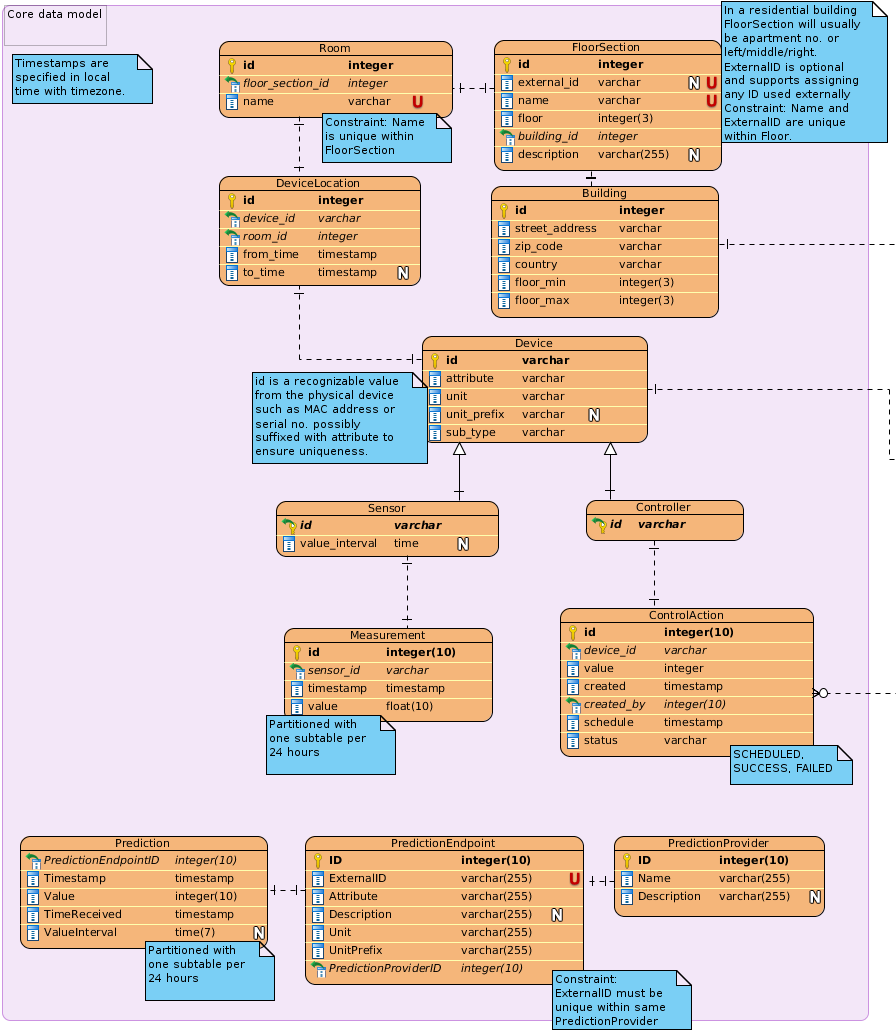
\includegraphics[width=\textwidth]{figures/db_core_schema}
    \caption{Database schema}
    \label{figureDbCoreModel}
\end{figure}

\section{Tables}

\subsection{Devices and measurements}

\paragraph{Device} 
Entries in \texttt{Device} correspond to physical control and sensor devices, with the modification that we store one logical device for each function of the physical device. Whether a device is a sensor or a controller is specified by its presence in table \texttt{Controller} or \texttt{Sensor}. Columns \texttt{Attribute}, \texttt{Unit} and \texttt{UnitPrefix} (such as milli) are for sensors specification of the incoming measurement values, while they for controllers specify the format of values to send to the controller when actuating it.

\paragraph{Sensor} 
Table \texttt{Sensor} specifies an optional property \texttt{ValueInterval} which is used when measurement values are aggregated over a limited time interval (such as 15 minutes). 

\paragraph{Measurement} 
Contains a row for each measurement received from a sensor. It simply consists of a \texttt{value}, a \texttt{timestamp} and a \texttt{sensor\_id}, which enables interpretation of the value. Column \texttt{exported} indicates whether a row has been exported to data warehouse or not.

The \texttt{Measurement} table is partitioned into subtables for each e.g. 24 hours. Querying the \texttt{Measurement} table will automatically retrieve data from all its subtables, while insertion must happen directly to the correct subtable. Each subtable has a constraint on the \texttt{timestamp}, preventing measurements from being entered in the wrong subtable.

\paragraph{ControlAction} 
Table \texttt{ControlAction} is intended to contain scheduled and past commands for controllers. An action is simply specified by a \texttt{value} which can be interpreted via the reference into table \texttt{Controller} and \texttt{Device}. Column \texttt{schedule} specifies the time for carrying out the action, and \texttt{status} indicates if execution is still pending or has been completed. Partitioning this table in the same way as table \texttt{Measurement} could be considered. In the current implementation of the VPP software, the \texttt{Controller} and \texttt{ControlAction} tables will always be empty.

\paragraph{Building, FloorSection, Room}
The physical properties of a building are modeled in these tables. A building consists of an integer range of floors. Each floor consists of \texttt{FloorSection}s which in most cases will be equivalent to apartments. The generalized term FloorSection is intended to support other types of buildings where designations such as "South wing" or other may be desired. Finally, a floor consists of named \texttt{Room}s. We do not expect to obtain device locations with a higher degree of accuracy than individual rooms.

\paragraph{DeviceLocation} This table maps \texttt{Device}s to \texttt{Room}s for specific time periods, indicating that devices may be moved around over time.

\subsection{Predictions}
While the data stored for predictions is quite similar to those for measurements, we have chosen to store them separately because of the fundamentally different semantics.

\paragraph{PredictionEndpoint} 
A logical source of predictions of one type. Specifies the \texttt{attribute} and \texttt{unit} of the incoming values and provides an optional \texttt{description}.

\paragraph{Prediction}
Actual prediction values. \texttt{timestamp} indicates the time for which the value applies, while \texttt{time\_received} indicates when the prediction was received from the provider. This is relevant since multiple predictions for the same future point in time may be received over time. Some values actually cover an interval (for instance predicted power consumption for a given day of 24 hours), which is specified in column \texttt{value\_interval}.
This table is partitioned in same way as table \texttt{Measurement}.


\section{CIM compliance}
Units, unit prefixes, timestamps and time durations are formatted to agree with CIM.

